\documentclass{article}
\usepackage{amsmath,graphicx,grffile}
\title{CLRS 15.2-5}
\author{Peter Danenberg}
\begin{document}
\maketitle

Full parenthesization maintains the multiplication tree property (see
figures \ref{fig:backbone} and \ref{fig:stacked} \emph{infra});
\emph{id est}, that a tree be a full binary tree where:

\begin{enumerate}
\item leaves are matrices and only matrices;
\item every parenthesis has two and only two children.
\end{enumerate}

Let $P(e) = n$ state that a fully parenthesized expression of $e$
elements requires $n$ pairs of parentheses.

\begin{description}
  \item[Basis:] $P(1) = 0$
  \item[Hypothesis:] $P(k) = k-1$
  \item[\emph{Praebendum:}] $P(k + 1) = k$
\end{description}

To insert a matrix into a multiplication tree of $k$ matrices,
resulting in a multiplication tree of $k+1$ matrices and while
maintaining the multiplication tree property; the matrix must be added
at a leaf by parenthesizing the leaf and adding itself and the new
node as children, resulting in $k$ pairs of parentheses.

Therefore:
\[(P(1)=0 \wedge (P(k)=k-1 \to P(k+1)=k)) \to \forall nP(n)=n-1\]

\begin{figure}[ht]
  \centering
  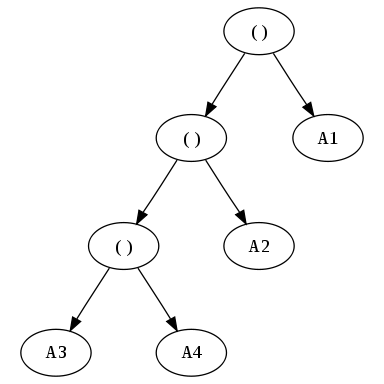
\includegraphics[width=0.5\linewidth]{15.2-5-backbone}
  \caption{Multiplication tree for $(A1 (A2 (A3 A4)))$}
  \label{fig:backbone}
\end{figure}

\begin{figure}[ht]
  \centering
  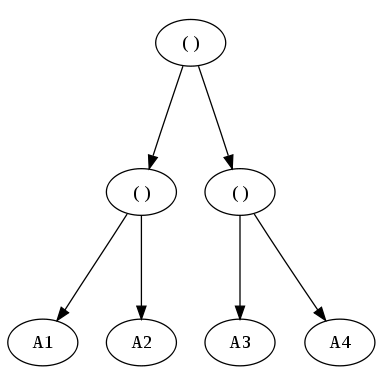
\includegraphics[width=0.5\linewidth]{15.2-5-stacked}
  \caption{Multiplication tree for $((A1 A2)(A3 A4))$}
  \label{fig:stacked}
\end{figure}
\end{document}
